\documentclass{article}

\usepackage{tikz}
\usepackage{verbatim}

\setlength\parindent{0pt}
\begin{document}
\pagestyle{empty}

\begin{comment}
    Examples of inversion graphs    
\end{comment}

% \foreach \a/\b/\c/\d in {
%     1/2/3/4, 1/2/4/3, 1/3/2/4, 1/3/4/2, 1/4/2/3, 1/4/3/2,
%     2/1/3/4, 2/1/4/3, 2/3/1/4, 2/3/4/1, 2/4/1/3, 2/4/3/1,
%     3/1/2/4, 3/1/4/2, 3/2/1/4, 3/2/4/1, 3/4/1/2, 3/4/2/1,
%     4/1/2/3, 4/1/3/2, 4/2/1/3, 4/2/3/1, 4/3/1/2, 4/3/2/1
%     } {
%     \begin{tikzpicture}[shorten >=1pt,-]
%         \tikzstyle{vertex}=[circle,draw=black,fill=white!25,minimum size=15pt,inner sep=0pt]
%         \foreach \num/\x in {\a/1, \b/2, \c/3, \d/4}
%                 \node[vertex] (V-\num) at (\x,0) {$\num$};

%             \foreach \from/\to in {\a/\b,\b/\c,\c/\d}
%                 \draw (V-\from) -- (V-\to);

%             \draw (V-\a) .. controls (1.5, 0.75) and (2.5, 0.75) .. (V-\c);
%             \draw (V-\a) .. controls (1.5, 1.5) and (3.5, 1.5) .. (V-\d);
%             \draw (V-\b) .. controls (2.5, 0.75) and (3.5, 0.75) .. (V-\d);
        
        
%     \end{tikzpicture}
% }


\begin{tikzpicture}[shorten >=1pt,-]
    \tikzstyle{vertex}=[circle,draw=black,fill=white!25,minimum size=15pt,inner sep=0pt]
    \foreach \num/\x in {1/1, 2/2, 3/3, 4/4}
            \node[vertex] (V-\num) at (\x,0) {$\num$};

        % \foreach \from/\to in {1/2,2/3,3/4}
        %     \draw (V-\from) -- (V-\to);

        % \draw (V-1) .. controls (1.5, 0.75) and (2.5, 0.75) .. (V-3);
        % \draw (V-1) .. controls (1.5, 1.5) and (3.5, 1.5) .. (V-4);
        % \draw (V-2) .. controls (2.5, 0.75) and (3.5, 0.75) .. (V-4);
\end{tikzpicture}
\\\\\\\\

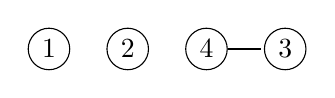
\begin{tikzpicture}[shorten >=1pt,-]
    \tikzstyle{vertex}=[circle,draw=black,fill=white!25,minimum size=15pt,inner sep=0pt]
    \foreach \num/\x in {1/1, 2/2, 4/3, 3/4}
            \node[vertex] (V-\num) at (\x,0) {$\num$};

        \foreach \from/\to in {4/3}
            \draw (V-\from) -- (V-\to);

        % \draw (V-1) .. controls (1.5, 0.75) and (2.5, 0.75) .. (V-3);
        % \draw (V-1) .. controls (1.5, 1.5) and (3.5, 1.5) .. (V-4);
        % \draw (V-2) .. controls (2.5, 0.75) and (3.5, 0.75) .. (V-4);
\end{tikzpicture}
\\\\\\\\


\begin{tikzpicture}[shorten >=1pt,-]
    \tikzstyle{vertex}=[circle,draw=black,fill=white!25,minimum size=15pt,inner sep=0pt]
    \foreach \num/\x in {1/1, 3/2, 2/3, 4/4}
            \node[vertex] (V-\num) at (\x,0) {$\num$};

        \foreach \from/\to in {3/2}
            \draw (V-\from) -- (V-\to);

        % \draw (V-1) .. controls (1.5, 0.75) and (2.5, 0.75) .. (V-3);
        % \draw (V-1) .. controls (1.5, 1.5) and (3.5, 1.5) .. (V-4);
        % \draw (V-2) .. controls (2.5, 0.75) and (3.5, 0.75) .. (V-4);
\end{tikzpicture}
\\\\\\\\

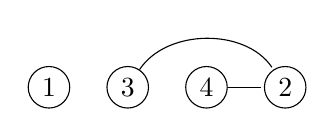
\begin{tikzpicture}[shorten >=1pt,-]
    \tikzstyle{vertex}=[circle,draw=black,fill=white!25,minimum size=15pt,inner sep=0pt]
    \foreach \num/\x in {1/1, 3/2, 4/3, 2/4}
            \node[vertex] (V-\num) at (\x,0) {$\num$};

        \foreach \from/\to in {4/2}
            \draw (V-\from) -- (V-\to);

        % \draw (V-1) .. controls (1.5, 0.75) and (2.5, 0.75) .. (V-3);
        % \draw (V-1) .. controls (1.5, 1.5) and (3.5, 1.5) .. (V-4);
        \draw (V-3) .. controls (2.5, 0.75) and (3.5, 0.75) .. (V-2);
\end{tikzpicture}
\\\\\\\\

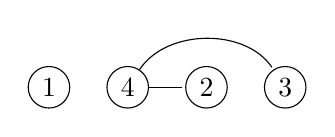
\begin{tikzpicture}[shorten >=1pt,-]
    \tikzstyle{vertex}=[circle,draw=black,fill=white!25,minimum size=15pt,inner sep=0pt]
    \foreach \num/\x in {1/1, 4/2, 2/3, 3/4}
            \node[vertex] (V-\num) at (\x,0) {$\num$};

        \foreach \from/\to in {4/2}
            \draw (V-\from) -- (V-\to);

        % \draw (V-1) .. controls (1.5, 0.75) and (2.5, 0.75) .. (V-3);
        % \draw (V-1) .. controls (1.5, 1.5) and (3.5, 1.5) .. (V-4);
        \draw (V-4) .. controls (2.5, 0.75) and (3.5, 0.75) .. (V-3);
\end{tikzpicture}
\\\\\\\\

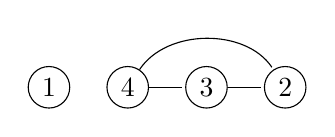
\begin{tikzpicture}[shorten >=1pt,-]
    \tikzstyle{vertex}=[circle,draw=black,fill=white!25,minimum size=15pt,inner sep=0pt]
    \foreach \num/\x in {1/1, 4/2, 3/3, 2/4}
            \node[vertex] (V-\num) at (\x,0) {$\num$};

        \foreach \from/\to in {4/3,3/2}
            \draw (V-\from) -- (V-\to);

        % \draw (V-1) .. controls (1.5, 0.75) and (2.5, 0.75) .. (V-3);
        % \draw (V-1) .. controls (1.5, 1.5) and (3.5, 1.5) .. (V-4);
        \draw (V-4) .. controls (2.5, 0.75) and (3.5, 0.75) .. (V-2);
\end{tikzpicture}
\\\\\\\\

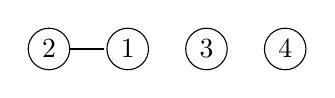
\begin{tikzpicture}[shorten >=1pt,-]
    \tikzstyle{vertex}=[circle,draw=black,fill=white!25,minimum size=15pt,inner sep=0pt]
    \foreach \num/\x in {2/1, 1/2, 3/3, 4/4}
            \node[vertex] (V-\num) at (\x,0) {$\num$};

        \foreach \from/\to in {2/1}
            \draw (V-\from) -- (V-\to);

        % \draw (V-1) .. controls (1.5, 0.75) and (2.5, 0.75) .. (V-3);
        % \draw (V-1) .. controls (1.5, 1.5) and (3.5, 1.5) .. (V-4);
        % \draw (V-2) .. controls (2.5, 0.75) and (3.5, 0.75) .. (V-4);
\end{tikzpicture}
\\\\\\\\

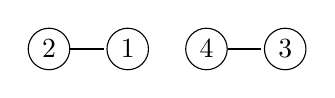
\begin{tikzpicture}[shorten >=1pt,-]
    \tikzstyle{vertex}=[circle,draw=black,fill=white!25,minimum size=15pt,inner sep=0pt]
    \foreach \num/\x in {2/1, 1/2, 4/3, 3/4}
            \node[vertex] (V-\num) at (\x,0) {$\num$};

        \foreach \from/\to in {2/1, 4/3}
            \draw (V-\from) -- (V-\to);

        % \draw (V-1) .. controls (1.5, 0.75) and (2.5, 0.75) .. (V-3);
        % \draw (V-1) .. controls (1.5, 1.5) and (3.5, 1.5) .. (V-4);
        % \draw (V-2) .. controls (2.5, 0.75) and (3.5, 0.75) .. (V-4);
\end{tikzpicture}
\\\\\\\\

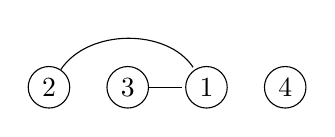
\begin{tikzpicture}[shorten >=1pt,-]
    \tikzstyle{vertex}=[circle,draw=black,fill=white!25,minimum size=15pt,inner sep=0pt]
    \foreach \num/\x in {2/1, 3/2, 1/3, 4/4}
            \node[vertex] (V-\num) at (\x,0) {$\num$};

        \foreach \from/\to in {3/1}
            \draw (V-\from) -- (V-\to);

        \draw (V-2) .. controls (1.5, 0.75) and (2.5, 0.75) .. (V-1);
        % \draw (V-1) .. controls (1.5, 1.5) and (3.5, 1.5) .. (V-4);
        % \draw (V-2) .. controls (2.5, 0.75) and (3.5, 0.75) .. (V-4);
\end{tikzpicture}
\\\\\\\\

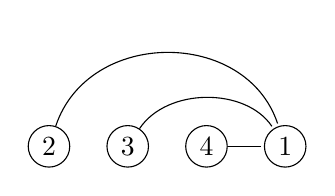
\begin{tikzpicture}[shorten >=1pt,-]
    \tikzstyle{vertex}=[circle,draw=black,fill=white!25,minimum size=15pt,inner sep=0pt]
    \foreach \num/\x in {2/1, 3/2, 4/3, 1/4}
            \node[vertex] (V-\num) at (\x,0) {$\num$};

        \foreach \from/\to in {4/1}
            \draw (V-\from) -- (V-\to);

        % \draw (V-1) .. controls (1.5, 0.75) and (2.5, 0.75) .. (V-3);
        \draw (V-2) .. controls (1.5, 1.5) and (3.5, 1.5) .. (V-1);
        \draw (V-3) .. controls (2.5, 0.75) and (3.5, 0.75) .. (V-1);
\end{tikzpicture}
\\\\\\\\

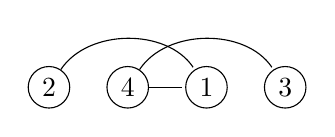
\begin{tikzpicture}[shorten >=1pt,-]
    \tikzstyle{vertex}=[circle,draw=black,fill=white!25,minimum size=15pt,inner sep=0pt]
    \foreach \num/\x in {2/1, 4/2, 1/3, 3/4}
            \node[vertex] (V-\num) at (\x,0) {$\num$};

        \foreach \from/\to in {4/1}
            \draw (V-\from) -- (V-\to);

        \draw (V-2) .. controls (1.5, 0.75) and (2.5, 0.75) .. (V-1);
        % \draw (V-1) .. controls (1.5, 1.5) and (3.5, 1.5) .. (V-4);
        \draw (V-4) .. controls (2.5, 0.75) and (3.5, 0.75) .. (V-3);
\end{tikzpicture}
\\\\\\\\

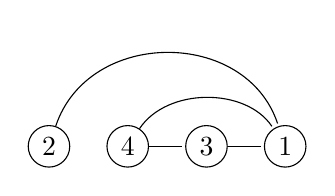
\begin{tikzpicture}[shorten >=1pt,-]
    \tikzstyle{vertex}=[circle,draw=black,fill=white!25,minimum size=15pt,inner sep=0pt]
    \foreach \num/\x in {2/1, 4/2, 3/3, 1/4}
            \node[vertex] (V-\num) at (\x,0) {$\num$};

        \foreach \from/\to in {4/3,3/1}
            \draw (V-\from) -- (V-\to);

        % \draw (V-1) .. controls (1.5, 0.75) and (2.5, 0.75) .. (V-3);
        \draw (V-2) .. controls (1.5, 1.5) and (3.5, 1.5) .. (V-1);
        \draw (V-4) .. controls (2.5, 0.75) and (3.5, 0.75) .. (V-1);
\end{tikzpicture}
\\\\\\\\

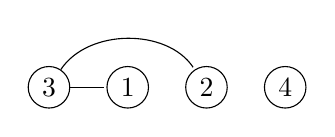
\begin{tikzpicture}[shorten >=1pt,-]
    \tikzstyle{vertex}=[circle,draw=black,fill=white!25,minimum size=15pt,inner sep=0pt]
    \foreach \num/\x in {3/1, 1/2, 2/3, 4/4}
            \node[vertex] (V-\num) at (\x,0) {$\num$};

        \foreach \from/\to in {3/1}
            \draw (V-\from) -- (V-\to);

        \draw (V-3) .. controls (1.5, 0.75) and (2.5, 0.75) .. (V-2);
        % \draw (V-1) .. controls (1.5, 1.5) and (3.5, 1.5) .. (V-4);
        % \draw (V-2) .. controls (2.5, 0.75) and (3.5, 0.75) .. (V-4);
\end{tikzpicture}
\\\\\\\\

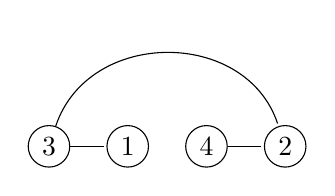
\begin{tikzpicture}[shorten >=1pt,-]
    \tikzstyle{vertex}=[circle,draw=black,fill=white!25,minimum size=15pt,inner sep=0pt]
    \foreach \num/\x in {3/1, 1/2, 4/3, 2/4}
            \node[vertex] (V-\num) at (\x,0) {$\num$};

        \foreach \from/\to in {3/1,4/2}
            \draw (V-\from) -- (V-\to);

        % \draw (V-1) .. controls (1.5, 0.75) and (2.5, 0.75) .. (V-3);
        \draw (V-3) .. controls (1.5, 1.5) and (3.5, 1.5) .. (V-2);
        % \draw (V-2) .. controls (2.5, 0.75) and (3.5, 0.75) .. (V-4);
\end{tikzpicture}
\\\\\\\\

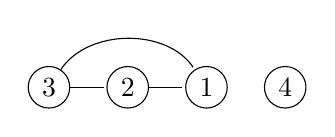
\begin{tikzpicture}[shorten >=1pt,-]
    \tikzstyle{vertex}=[circle,draw=black,fill=white!25,minimum size=15pt,inner sep=0pt]
    \foreach \num/\x in {3/1, 2/2, 1/3, 4/4}
            \node[vertex] (V-\num) at (\x,0) {$\num$};

        \foreach \from/\to in {3/2,2/1}
            \draw (V-\from) -- (V-\to);

        \draw (V-3) .. controls (1.5, 0.75) and (2.5, 0.75) .. (V-1);
        % \draw (V-1) .. controls (1.5, 1.5) and (3.5, 1.5) .. (V-4);
        % \draw (V-2) .. controls (2.5, 0.75) and (3.5, 0.75) .. (V-4);
\end{tikzpicture}
\\\\\\\\

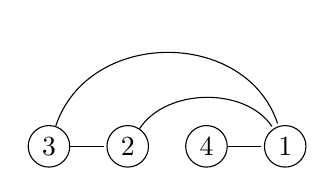
\begin{tikzpicture}[shorten >=1pt,-]
    \tikzstyle{vertex}=[circle,draw=black,fill=white!25,minimum size=15pt,inner sep=0pt]
    \foreach \num/\x in {3/1, 2/2, 4/3, 1/4}
            \node[vertex] (V-\num) at (\x,0) {$\num$};

        \foreach \from/\to in {3/2,4/1}
            \draw (V-\from) -- (V-\to);

        % \draw (V-1) .. controls (1.5, 0.75) and (2.5, 0.75) .. (V-3);
        \draw (V-3) .. controls (1.5, 1.5) and (3.5, 1.5) .. (V-1);
        \draw (V-2) .. controls (2.5, 0.75) and (3.5, 0.75) .. (V-1);
\end{tikzpicture}
\\\\\\\\

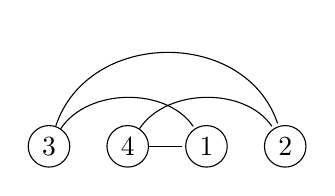
\begin{tikzpicture}[shorten >=1pt,-]
    \tikzstyle{vertex}=[circle,draw=black,fill=white!25,minimum size=15pt,inner sep=0pt]
    \foreach \num/\x in {3/1, 4/2, 1/3, 2/4}
            \node[vertex] (V-\num) at (\x,0) {$\num$};

        \foreach \from/\to in {4/1}
            \draw (V-\from) -- (V-\to);

        \draw (V-3) .. controls (1.5, 0.75) and (2.5, 0.75) .. (V-1);
        \draw (V-3) .. controls (1.5, 1.5) and (3.5, 1.5) .. (V-2);
        \draw (V-4) .. controls (2.5, 0.75) and (3.5, 0.75) .. (V-2);
\end{tikzpicture}
\\\\\\\\

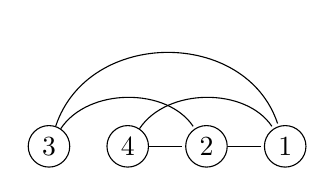
\begin{tikzpicture}[shorten >=1pt,-]
    \tikzstyle{vertex}=[circle,draw=black,fill=white!25,minimum size=15pt,inner sep=0pt]
    \foreach \num/\x in {3/1, 4/2, 2/3, 1/4}
            \node[vertex] (V-\num) at (\x,0) {$\num$};

        \foreach \from/\to in {4/2,2/1}
            \draw (V-\from) -- (V-\to);

        \draw (V-3) .. controls (1.5, 0.75) and (2.5, 0.75) .. (V-2);
        \draw (V-3) .. controls (1.5, 1.5) and (3.5, 1.5) .. (V-1);
        \draw (V-4) .. controls (2.5, 0.75) and (3.5, 0.75) .. (V-1);
\end{tikzpicture}
\\\\\\\\

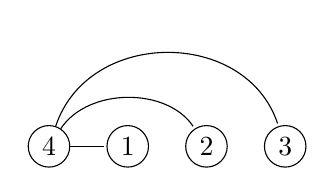
\begin{tikzpicture}[shorten >=1pt,-]
    \tikzstyle{vertex}=[circle,draw=black,fill=white!25,minimum size=15pt,inner sep=0pt]
    \foreach \num/\x in {4/1, 1/2, 2/3, 3/4}
            \node[vertex] (V-\num) at (\x,0) {$\num$};

        \foreach \from/\to in {4/1}
            \draw (V-\from) -- (V-\to);

        \draw (V-4) .. controls (1.5, 0.75) and (2.5, 0.75) .. (V-2);
        \draw (V-4) .. controls (1.5, 1.5) and (3.5, 1.5) .. (V-3);
        % \draw (V-2) .. controls (2.5, 0.75) and (3.5, 0.75) .. (V-4);
\end{tikzpicture}
\\\\\\\\

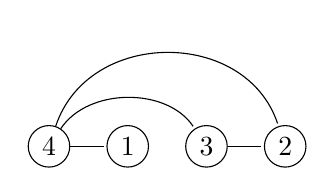
\begin{tikzpicture}[shorten >=1pt,-]
    \tikzstyle{vertex}=[circle,draw=black,fill=white!25,minimum size=15pt,inner sep=0pt]
    \foreach \num/\x in {4/1, 1/2, 3/3, 2/4}
            \node[vertex] (V-\num) at (\x,0) {$\num$};

        \foreach \from/\to in {4/1, 3/2}
            \draw (V-\from) -- (V-\to);

        \draw (V-4) .. controls (1.5, 0.75) and (2.5, 0.75) .. (V-3);
        \draw (V-4) .. controls (1.5, 1.5) and (3.5, 1.5) .. (V-2);
        % \draw (V-2) .. controls (2.5, 0.75) and (3.5, 0.75) .. (V-4);
\end{tikzpicture}
\\\\\\\\

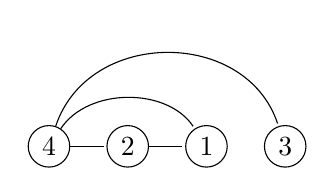
\begin{tikzpicture}[shorten >=1pt,-]
    \tikzstyle{vertex}=[circle,draw=black,fill=white!25,minimum size=15pt,inner sep=0pt]
    \foreach \num/\x in {4/1, 2/2, 1/3, 3/4}
            \node[vertex] (V-\num) at (\x,0) {$\num$};

        \foreach \from/\to in {4/2,2/1}
            \draw (V-\from) -- (V-\to);

        \draw (V-4) .. controls (1.5, 0.75) and (2.5, 0.75) .. (V-1);
        \draw (V-4) .. controls (1.5, 1.5) and (3.5, 1.5) .. (V-3);
        % \draw (V-2) .. controls (2.5, 0.75) and (3.5, 0.75) .. (V-4);
\end{tikzpicture}
\\\\\\\\

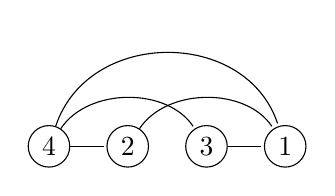
\begin{tikzpicture}[shorten >=1pt,-]
    \tikzstyle{vertex}=[circle,draw=black,fill=white!25,minimum size=15pt,inner sep=0pt]
    \foreach \num/\x in {4/1, 2/2, 3/3, 1/4}
            \node[vertex] (V-\num) at (\x,0) {$\num$};

        \foreach \from/\to in {4/2, 3/1}
            \draw (V-\from) -- (V-\to);

        \draw (V-4) .. controls (1.5, 0.75) and (2.5, 0.75) .. (V-3);
        \draw (V-4) .. controls (1.5, 1.5) and (3.5, 1.5) .. (V-1);
        \draw (V-2) .. controls (2.5, 0.75) and (3.5, 0.75) .. (V-1);
\end{tikzpicture}
\\\\\\\\

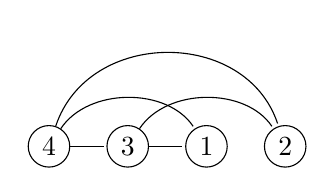
\begin{tikzpicture}[shorten >=1pt,-]
    \tikzstyle{vertex}=[circle,draw=black,fill=white!25,minimum size=15pt,inner sep=0pt]
    \foreach \num/\x in {4/1, 3/2, 1/3, 2/4}
            \node[vertex] (V-\num) at (\x,0) {$\num$};

        \foreach \from/\to in {4/3,3/1}
            \draw (V-\from) -- (V-\to);

        \draw (V-4) .. controls (1.5, 0.75) and (2.5, 0.75) .. (V-1);
        \draw (V-4) .. controls (1.5, 1.5) and (3.5, 1.5) .. (V-2);
        \draw (V-3) .. controls (2.5, 0.75) and (3.5, 0.75) .. (V-2);
\end{tikzpicture}
\\\\\\\\

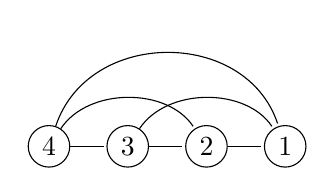
\begin{tikzpicture}[shorten >=1pt,-]
    \tikzstyle{vertex}=[circle,draw=black,fill=white!25,minimum size=15pt,inner sep=0pt]
    \foreach \num/\x in {4/1, 3/2, 2/3, 1/4}
            \node[vertex] (V-\num) at (\x,0) {$\num$};

        \foreach \from/\to in {4/3, 3/2, 2/1}
            \draw (V-\from) -- (V-\to);

        \draw (V-4) .. controls (1.5, 0.75) and (2.5, 0.75) .. (V-2);
        \draw (V-4) .. controls (1.5, 1.5) and (3.5, 1.5) .. (V-1);
        \draw (V-3) .. controls (2.5, 0.75) and (3.5, 0.75) .. (V-1);
\end{tikzpicture}
\\\\\\\\


\end{document}